\section{Bottlenecks and trade--offs}

  With extremely efficient FFT and point--wise product the ConvNet
  inference becomes memory throughput bound.

  Let's consider the three/four stages: 1/2) FFT of inputs/kernels,
  point--wise madds and iFFT of outputs.  Each of the stages is
  actually memory bound on the Xeon Phi, especially because of the
  lack of L3 cache that is shared among the CPUs.

  KNL has MDCRAM with 500 GB/s bandwidth and 6 TFLOP/s of single
  precision computing power.  500 GB/s is equivalent to 500/8 Gfloats
  (32-bit floats) per second = 62.5 Gfloats/s.  To be able to
  optimally utilize the VPUs, we need at least $6000/62.5 \approx 100$
  operations per float fetched from MDCRAM.

\section{1D ConvNet}

  We explain how to perform the forward pass on a 1D ConvNet first.
  We'll explain how an ND ConvNet can be converted into a set of 1D
  ConvNets.

  Let's consider a convolutional layer with $f$ input and $f'$ output
  channels.  Let $V$ be the size (in floats) of the vector registers
  available.  In the case of Xeon Phi, $V=16$.  Further, let's assume
  that both $f$ and $f'$ are divisible by $V$.  This is true for most
  modern networks.  When $f$ and $f'$ are not divisible by $V$, it is
  always possible to add extra ``dummy'' channels.

  Let the image size be $x$ and kernel size $k$.  Also, assume the
  batch size of $b$.

  We'll assume that $x$ is either 32, 64 or 128 (the best choice
  should be empirically determined).  This is b/c fast FFT algorithms
  exist for such sizes.

  When $x$ has a different size, it is always possible to either pad
  it (if it's smaller).  Or divide it into overlapping intervals
  (overlap by kernel size) such that each interval produces part of
  the output.  Effectively, dividing $x$ into $n$ intervals, increases
  the batch size by a factor of $n$.  Therefore we'd be solving the
  same problem with a larger batch size $b' = bn$.

  \subsection{Goals}

  The main goal of the algorithm is to increase flops to memory
  bandwidth ratio.  This means that we'd like to re-use L1 and L2
  cache as much as possible, as well as the register file.

  Xeon Phi physical core has $32$ zmm registers (each is $512$ bits =
  $64$ bytes).  Total register file is then $2KB$.  It also has $32KB$
  of L1 instruction cache and $32KB$ of L1 data cache.  It also has
  $1MB$ of L2 cache.

  The register file, as well as the caches are shared among hardware
  threads, effectively lowering available amount per thread.  For
  simplicity, we'll assume using $4$ threads per core, but similar
  analysis can be performed when using less cores.

  In this case, each thread has $8$ available registers, $8KB$ of L1
  and $256KB$ of L2 cache available.

  \subsection{Algorithm}

  The algorithm divides the input and output channels into sets of
  $V$.  This is done in order to use the zmm registers.

  The input tensor of size $b \times f \times x$ is reshaped into a
  tensor of size $b \times (f / V) \times x \times V$.  Such that the
  element $(i,j,k,l)$ of the new tensor corresponds to the element
  $(i,j*V+l,k)$ of the original one.  The output tensor will be shaped
  in similar fashion.

  The kernels tensor of size $f' \times f \times k$ is reshaped to a
  tensor of size $(f'/V) \times (f / V) \times V \times k \times V$
  such that an element $(i,j,k,l,m)$ of the new tensor corresponds to
  $(i*V+m,j*V+k,l)$

  In the first step of the algorithm, FFTs of all the inputs are
  computed.  This will be memory bound, and can hardly be improved as
  we'll discuss later.  However, the amount of computation required
  here is much less than following main loop that performs pointwise
  products.

  The input shape of the transformed algorithm will then be $b \times
  (f/V) \times x \times 2 \times V$.  The $2$ comes from the fact that
  we need complex numbers.

  The algorithm then loops over output sets of channels, and then for
  each output set, it loops over the input sets of channels.


  \begin{algorithm}
      \begin{codebox}
        \Procname{$\proc{inner-loop}(in,ker,out,f,len)$}
        \li \For $i \gets 0 \To len-1$
        \li \Do  $out[i][0][:] = \proc{FMSUB}( ker[i][1][:], in[i][1][f], out[i][0][:] )$
        \li      $out[i][0][:] = \proc{FMSUB}( ker[i][0][:], in[i][0][f], out[i][0][:] )$
        \li      $out[i][1][:] = \proc{FMADD}( ker[i][1][:], in[i][0][f], out[i][1][:] )$
        \li      $out[i][1][:] = \proc{FMADD}( ker[i][0][:], in[i][1][f], out[i][1][:] )$
        \End
      \end{codebox}
    \caption{Innermost loop.}
    \label{alg:cpu_direct}
  \end{algorithm}



  \begin{algorithm}
      \begin{codebox}
        \Procname{$\proc{inner-loop}(in,ker,out,x)$}
        \li $L1 \gets \proc{L1-cache-tensor}[x][2][V]$
        \li \For $f \gets 0 \To V$
        \li \Do  $L1 \gets \proc{Expand-and-FFT}(ker[f][:][:])$
        \li      \For $i \gets 0 \To b$
        \li      \Do  $\proc{inner-loop}(in,L1,out,f,x)$
        \End \End
      \end{codebox}
    \caption{Algorithm loop.}
    \label{alg:cpu_direct}
  \end{algorithm}

  From the algorithm we can see that $x \times 2 \times V$ has to fit
  in L1 cache, when $V=16$, $x$ is limited to $64$.  Also, in and out
  have to fit in L2 cache. limiting $b$ to $32$.  We could also limit
  $x$ to $32$, allowing $b$ up to $32$.  This should also be
  empirically determined.

  Now, let's count total transfers from and to main memory to L2 of
  the algorithm.  We fetch the in tensor, and store out tensor.  Note
  that the out tensor could be re--used in the next iteration over
  input feature maps, thus this is the worst case.  total transfer is
  then $b \times x \times 2 \times V$ for both input and output.  That
  is total of  $2xbV$.  Total transfer for kernels is $kV^2$.

  Now, let's count number of flops.  Each FMADD and FMSUB perform 32
  flops (16 muls and 16 ads).  the FFT of size x performs approx $5(x
  \log x)V$ flops.

  Hence ratio of flops to bandwidth is

  $$ \frac{ V \cdot 5x \log x + V \cdot b \cdot 4x \cdot 32 }{2xbV + kV^2}$$


  $$ \frac{ 5x \log x + b \cdot 4x \cdot 32 }{2xb + kV}$$

  For $b = 64$ and $x = 32$ we get approximately $48 FLOPS$ per a
  floating point, or $6$ flops per byte.  With the memory bandwidth of
  approx $500 GB/s$, we can get at most $3 TFLOP/s$


  In order to improve the possible utilization, we must consider
  different subdivision into problems.  Mainly, we will increase the
  size of the sets of input and output sets to $2V = 32$ channels.
  This will decrease the maximal size of $b$ and $x$ to the one such
  that $b\times v \le 32^2$.

  This way we can theoretically utilize all $6 TFLOP/s$ available.


\section{Algorithm Details}

  Ignoring the FFTs of the inputs, which can be amortized out during
  the first pass of the pointwise-mult algorithm.

  Assume we keep $N$ output sets.  An output set has $b \times x
  \times V$ complex numbers, which is $32bx$ floats.

  Then, for each fetched input set of $32bx$ floats we need to:

  \begin{enumerate}
    \item Fetch kernels $2k \times 16^2$ floats.
    \item Perform FFTs of all kernels
    \item Do pointwise mults
  \end{enumerate}

  Additional fetches include $2k \times 16^2$.

  Total number of FLOPS (excluding FFTs of the fetched kernels).  Is
  $32N$ per fetched float.

  To have $> 100$ FLOPS per fetched float, we need $N \ge 4$.

  This means keeping 5 sets in L2.

  A set requires $32bx$ memory.  So we need $160bx$ floats to fit in
  $256$ KB of L2.  Which means $bx \le 400$.  $x$ has to be either 16
  or 32.  If 16, then $b \le 25$.  If 32, then $b \le 12$.

  Alternatively, we could use 2 threads per core, to increase the
  amount of available cache.



\section{Pointwise-mult analysis}

  Assume collecting $N$ sets of outputs.  Each output set is of size
  $b \times x \times 16$.

  We then fetch an input set of $16bx$ complex numbers.  Total memory
  in L2 required is $16(N+1)bx$ complex numbers.  Total kernels
  elements that have to be fetched $256Nk$, however we fetch only
  $16k$ at the time.

  So, total complex numbers fetched is:

  $$16bx + 256Nk$$

  We will ignore the FFT computation of kernels (underestimate FLOPS
  per byte).

  Each complex number of the input gets $16N$ MADDS to the output.
  Total complex MADDs then is:

  $$256Nbx$$

  Now let's find the ration of FLOPS performed vs Memory fetched.

  $8$ FLOPS per complex MADD (4 floating point MADDs).  Total of
  $4096Nbx$ FLOPS.

  Fetched memory is ($8$ bytes per complex num)

  $$128bx + 2048Nk$$

  If $128bx > 2048Nk$ we get

  $$\frac{4096Nbx}{256bx} = 16N$$

  FLOPs per byte.  Otherwise, we get

  $$\frac{bx}{k}$$

  Our constraint is that $16(N+1)bx$ complex numbers has to fit in L2.
  So,

  $$128(N+1)bx \le L_2$$

  Allowing for $256$ KB of L1, we get

  $$(N+1)bx \le 2048$$

  \subsection{Peak FLOPs and bandwidth}

  The Xeon Phi has $64$ cores, each with 2 FMAs, capable of $32$ FLOPS
  per cycle (fmadd on zmm).  That is total of $4096$ FLOPS per cycle.
  The clock is at 1.3 GHz, giving us $5324.8$ GFLOP/s


  The MDCRAM memory throughput is $500$ GB/s.  To fully utilize the
  system, we need to perform $11$ FLOPs for each byte fetched from
  memory.  This is the same as performing $44$ flops for each float
  fetched from memory.

  So we want both

  $$16N \ge 11$$

  And,

  $$bx \ge 11k$$

  From the memory requirement we also have

  $$(N+1)bx \le 2048$$

  $$bx \le \frac{2048}{N+1}$$

  $$11k \le \frac{2048}{N+1}$$

  $$k \le \frac{186}{N+1}$$

  Which should always work.

  We can also derrive

  $$16(N+1) \ge 27$$

  $$N+1 \ge 1.7$$

  $$bx \le 1200$$

\section{Notes - TODO}

  Reduced FLOP fft of kernels to $O(k \log n)$. It is definitely
  possible with Radix-2 approach.

  In the template loop to $\min{K, N/2}$.  With $\log N$ recursive
  steps, $K \log N$ is achievable.





  \begin{algorithm}

      \begin{codebox}
        \Procname{$\proc{inner-loop<Len,F>}(in,ker,out)$}
        \li \For $i \gets 0 \To len-1$
        \li \Do  $out[i,0,:] = \proc{fmadd}( ker[i,0,:], in[i,0,F], out[i,0,:] )$
        \li      $out[i,0,:] = \proc{fnmadd}( ker[i,1,:], in[i,1,F], out[i,0,:] )$
        \li      $out[i,1,:] = \proc{fmadd}( ker[i,0,:], in[i,1,F], out[i,1,:] )$
        \li      $out[i,1,:] = \proc{fmadd}( ker[i,1,:], in[i,0,F], out[i,1,:] )$
        \End
      \end{codebox}

      \begin{codebox}
        \Procname{$\proc{output-loop<B,Len,K>}(in,ker,out,l1cache)$}
        \li \For $F \gets 0 \To 15$
        \li \Do  \For $k \gets 0 \To K-1$
        \li      \Do  $l1cache[k,0,:] = ker[F,k,0,:]$
        \li           $l1cache[k,1,:] = ker[F,k,1,:]$
                  \End
        \li $\proc{FFT<Len,K>}(l1cache)$
        \li \For $i \gets 0 \To B-1$
        \li \Do  $\proc{batch-loop<Len,F>}(in[b,:,:,:],l1cache,out[b,:,:,:])$
        \End
        \End
      \end{codebox}

      \begin{codebox}
        \Procname{$\proc{multi-output-loop<N,B,Len,K>}(in,ker,out,l1cache)$}
        \li \For $i \gets 0 \To N$
        \li \Do  $\proc{output-loop<B,Len,K>}(in,ker[i,:,:,:,:],out[i,:,:,:,:])$
        \End
      \end{codebox}



    \caption{Innermost loop.}
  \end{algorithm}

  \section{About KNL}

  \begin{figure}
    \begin{center}
      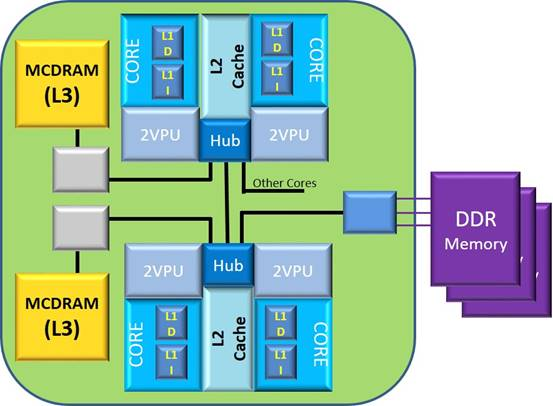
\includegraphics[width=0.97\linewidth]{fig/knl.jpg}
    \end{center}
    \caption{KNK CPU design.}
    \label{fig:knl}
  \end{figure}



  \section{Special Cases}

  Note that, in order to fit L1, $x$ has to be $\le 64$.

  \subsection{$x=32$}

  For $x=32$, we need $4096(N+1)b$ bytes in $L2$ at the time.  Limiting L2 to $256k$ we get $(N+1)b \le 64$.  Choices are either $N=2$, and
